\chapter{Introduction}\label{ch:introduction}


\begin{chapquote}{Henri Poincaré}
La mathématique est l'art de donner le même nom à des choses différentes.
\end{chapquote}

\lipsum[1-3]
\gls{mse}

Textwidth: \printlength{\textwidth}

\begin{figure}
    \centering
    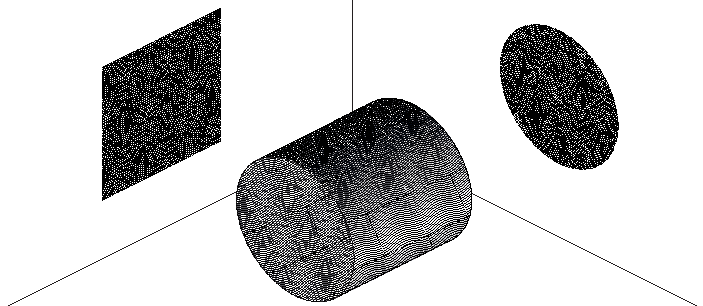
\includegraphics{cylinder.pdf}
    \caption[Cylinder projected as a circle and a square.]{A same object can have different representations. Depending on the projection, a cylinder can be viewed either as a square or as a circle.}
\end{figure}



%%%%%%%%%%%%%%%%%%%%%%%%%%%%%%%%%%%%%%%%%%%%%%%%%%
% Keep the following \cleardoublepage at the end of this file, 
% otherwise \includeonly includes empty pages.
\cleardoublepage

% vim: tw=70 nocindent expandtab foldmethod=marker foldmarker={{{}{,}{}}}
